\chapter{Result analysis}
This chapter shows the quantitative and qualitative analysis of the images generated from using different approaches.


\section{Dataset}
All the experimental work was carried out on the Kvasir Capsule Endoscopy Dataset\cite{data}. A segment of Kvasir-Capsule, a video capsule endoscopy data set, is used for this project.
Each image has 336x336 dimensions and is in RGB colour code. There are total of 47236 images belonging to different sub-categories of medical anomalies.
The original dataset had the images as shown in Table \ref{Table:4.1}
\begin{table}[h!]
\centering
\caption{Table of original data set.}
\begin{tabular}{ |c|c| }
\hline
 Normal clean mucosa & 34338 \\
 Ileocecal valve & 4189 \\
 Reduced mucosal view & 2096 \\
 Pylorus    &    1529 \\
 Angiectasia         &     866 \\
 ulcer               &     854 \\
 Foreign body        &     766\\    
 Lymphangiectasia    &     592 \\
 Erosion             &     506 \\
 Blood - fresh       &     446 \\
 Erythema            &      159 \\
 Polyp               &      55 \\
 Blood - hematin     &       12 \\
 ampulla of water    &        10 \\
\hline
\end{tabular}
\label{Table:4.1}
\end{table}
\newline
The Experimentation was carried on multiple subsets of the original Dataset.
Initially 10,000 training images were randomly sampled from the original set with 1000 testing images. Few sample images from the dataset are given in Fig.\ref{fig:label4.1}
\begin{figure}[h]
    \centering
    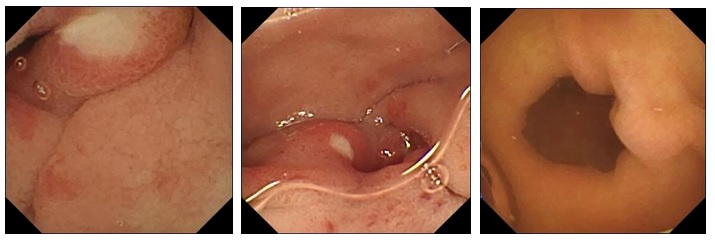
\includegraphics[totalheight=1.5in]{Chapter4/Fig4.1.jpg}
    \caption[Glimpse of uncropped capsule images]{Glimpse of uncropped capsule images.\cite{data}}
    \label{fig:label4.1}
\end{figure}
\newpage
As we can see in the sample images Fig.\ref{fig:label4.1} that the corner of the images are complete black spaces, while feeding this data to the image super resolution network for learning purposes, the network was not able to learn well and an semi transparent white layer was observed on the output images. To overcome this problem, we feed the network with cropped images, that didn't have any blank spot in the corners.
The glimpse of that dataset is shown in Fig.\ref{fig:label4.2}
\begin{figure}[h]
    \centering
    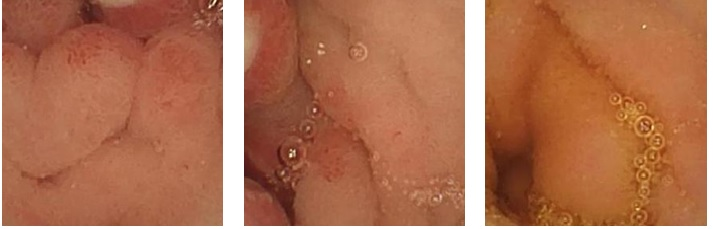
\includegraphics[totalheight=1.5in]{Chapter4/Fig4.2.jpg}
    \caption[Glimpse of Cropped dataset]{Glimpse of Cropped dataset.\cite{data}}
    \label{fig:label4.2}
\end{figure}
\newline
As Image super resolution is a comperatively complex task, the network was not able to perform well when the input data belonged to multiple classes, as the underlying spartial information was different for different classes. Hence a new dataset was developed which was the subset of original dataset of cropped images.
The final training of all the models/networks was done on this dataset. After cropping, the resolution of the cropped images is $228 \times 228$ pixels, which was $336 \times 336$ pixels originally.
\section{Experimental analysis on SOTA models}
To set the basline for the proposed model, we trained the existing state of art models with our dataset and generated the results using those models, the results are shown in following subsections.
\subsection{Training Details of SRGAN}
On an NVIDIA Tesla GPU, we trained each network using 10,000 photos from the Kvasir Dataset\cite{data}. Compared to the test images, these pictures are different. By employing a bicubic kernel and a downsampling factor of x4, we were able to derive the LR images from the HR images (BGR, C = 3). Randomly select 16 HR subimages of size 96x96 from various training images for each mini-batch were selected. It should be noted that since the generator model is completely convolutional, it may be applied to images of any size. The HR picture was scaled in range to [1,1] and the LR input image range to [0,1]. In order to determine the MSE loss, pictures with an intensity range of [1,1] were used. In order to get VGG losses on a par with MSE losses, VGG feature maps were additionally rescaled by a factor of 11.25 percentage. This is equal to adding a rescaling factor of 0.006. The Adam optimizer \cite{Adam} was used  with 1 = 0.9 for optimization. The SRResNet networks were trained using 106 update iterations and a learning rate of 0.0001. To prevent undesirable local optima, They learned MSE-based SRResNet network as initialization for the generator when training the actual GAN. A total of 105 update iterations at a learning rate of 104 and an additional 105 iterations at a slower rate of 105 were used to train all SRGAN versions. We alternate the updates to the discriminator and generator networks, which is equal to GAN's\cite{GAN} k = 1. 
\subsection{Result of SRGAN}
The model was trained at the above mentioned parameters and the below mentioned results were obtained. The PSNR of SRGAN for cropped data was recorded as 37.217 dB which is comparatively better compared to Bicubically upsampled image having PSNR of 37.1 dB , while that for uncropped data was recorded as 36.396 dB which is comparatively better compared to Bicubically upsampled image having PSNR of 35.36 dB. SSIM score was also increased compared to the Bicubically upsampled images.
The details of SSIM and PSNR for cropped as well as uncropped images is shown in table \ref{Table:5.1}. And the output results can be seen in Fig. \ref{fig:label5.2}.
\begin{table}[h!]
\centering
\caption{PSNR and SSIM for SRGAN.}
\begin{tabular}{ |c|c|c|c| }
\hline
 Method & PSNR(dB) & SSIM(dB) & Dataset \\ 
  \hline
 BICUBIC &	35.36 &	0.88 & uncropped \\
 SRGAN &	36.396 &	0.9083 & uncropped \\
 BICUBIC &	37.26 &	0.9 & cropped \\
 SRGAN &	37.06	& 0.9 & cropped\\
\hline
\end{tabular}
\label{Table:5.1}
\end{table}
\newline


\begin{figure}[H]
    \centering
        \begin{subfigure}[b]{0.275\textwidth}
    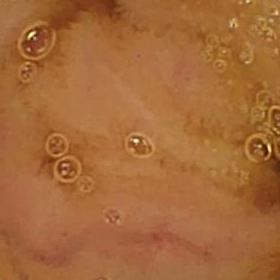
\includegraphics[width=\textwidth]{Chapter7/hr_9.jpg}
    \caption{HR}
  \end{subfigure}
  \begin{subfigure}[b]{0.275\textwidth}
    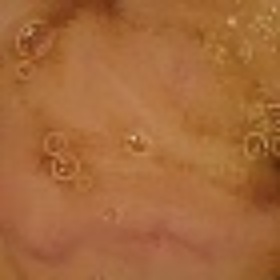
\includegraphics[width=\textwidth]{Chapter7/Bicubic_9.jpg}
    \caption{Bicubic}
  \end{subfigure}
  \begin{subfigure}[b]{0.275\textwidth}
    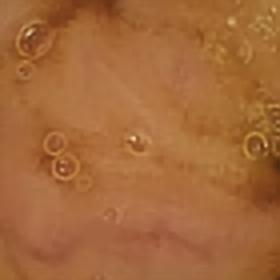
\includegraphics[width=\textwidth]{Chapter7/srgan_9.jpg}
    \caption{SRGAN}
  \end{subfigure}
  
  \begin{subfigure}[b]{0.275\textwidth}
    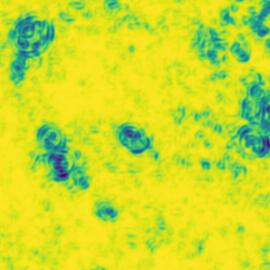
\includegraphics[width=\textwidth]{Chapter7/SSIM_bicubic_9.jpg}
    \caption{HR-Bicubic}
  \end{subfigure}
  \begin{subfigure}[b]{0.275\textwidth}
    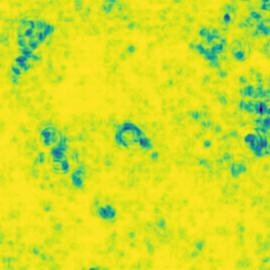
\includegraphics[width=\textwidth]{Chapter7/SSIM_srgan_9.jpg}
    \caption{HR-SRGAN}
  \end{subfigure}
    \caption{SRGAN Generated Image and their SSIM maps: (1) HR image (2) Bicubic Interpolated image (3) SR image (4)  SSIM-map (HR-Bicubic) (5)SSIM-map (HR-SR).\cite{DenseNET} \cite{SSIM}}
    \label{fig:label5.2}
\end{figure}

\subsection{Training Details of CycleGAN}
Training details We apply two techniques from recent works to stabilize our model training procedure. First, for $L_{G A N}$, we replace the negative log likelihood objective by a least-squares loss. This loss is more stable during training and generates higher quality results. In particular, for a GAN loss $L_{G A N}$(G,D,X,Y ), we train the G to minimize the loss and train the Discriminator.
Second, to reduce model oscillation , they update the discriminators using a history of generated images rather than the ones produced by the latest generators. We keep an image buffer that stores the 50 previously created images. For all the experiments, We use the Adam solver \cite{Adam} 
with a batch size of 1. All networks were trained from scratch with a learning rate of 0.0002. We keep the same learning rate for the first 100 epochs and linearly decay the rate to zero over the next 100 epochs.
\subsection{Results for CycleGAN}
The model was trained at the above mentioned parameters and the below mentioned results were obtained. The PSNR of CycleGAN for cropped data was recorded as 36.9 dB which is comparatively better compared to Bicubically upsampled image having PSNR of 37.1 dB , while that for uncropped data was recorded as 36.3 dB which is comparatively better compared to Bicubically upsampled image having PSNR of 37.1 dB. SSIM score was also increased compared to the Bicubically upsampled images.
The details of SSIM and PSNR for cropped as well as uncropped images is shown in Table \ref{Table:5.2}
\begin{table}[H]
\centering
\caption{PSNR and SSIM for CycleGAN.}
\begin{tabular}{ |c|c|c|c| }
\hline
 Method & PSNR(dB) & SSIM(dB) & Dataset \\ 
  \hline
 BICUBIC &	37.1 &	0.88 & uncropped \\
 CycleGAN &	36.3 &	0.9123 & uncropped \\
 BICUBIC &	36.9 &	0.89 & cropped \\
 CycleGAN &	37.1	& 0.9123 & cropped\\
\hline
\end{tabular}
\label{Table:5.2}
\end{table}

\begin{figure}[H]
    \centering
        \begin{subfigure}[b]{0.275\textwidth}
    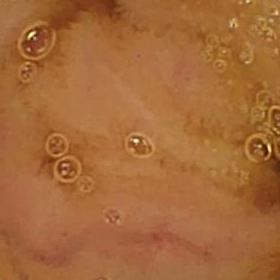
\includegraphics[width=\textwidth]{Chapter7/hr_9.jpg}
    \caption{HR}
  \end{subfigure}
  \begin{subfigure}[b]{0.275\textwidth}
    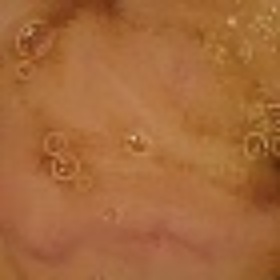
\includegraphics[width=\textwidth]{Chapter7/Bicubic_9.jpg}
    \caption{Bicubic}
  \end{subfigure}
  \begin{subfigure}[b]{0.275\textwidth}
    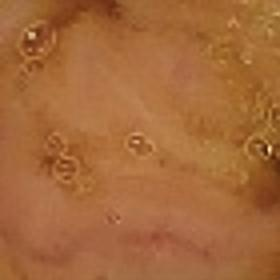
\includegraphics[width=\textwidth]{Chapter7/cycle_mse_9.jpg}
    \caption{CycleGAN}
  \end{subfigure}
  
  \begin{subfigure}[b]{0.275\textwidth}
    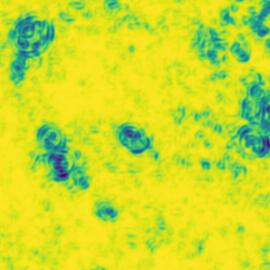
\includegraphics[width=\textwidth]{Chapter7/SSIM_bicubic_9.jpg}
    \caption{HR-Bicubic}
  \end{subfigure}
  \begin{subfigure}[b]{0.275\textwidth}
    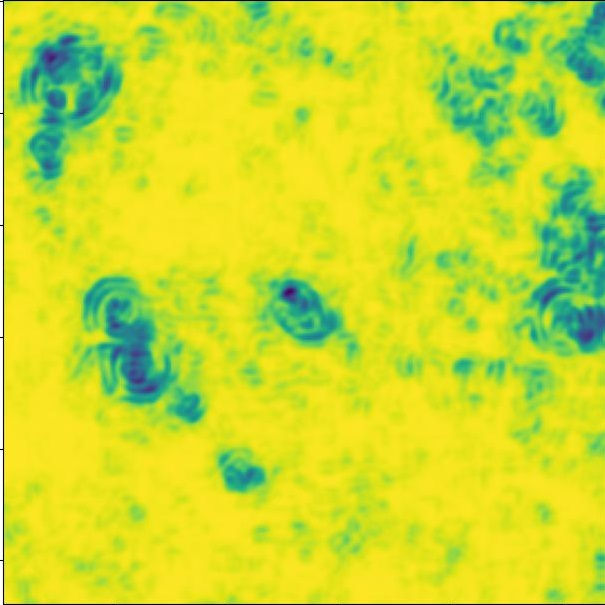
\includegraphics[width=\textwidth]{Chapter5/SSIM_cyclegan_9.jpg}
    \caption{HR-CycleGAN}
  \end{subfigure}
    \caption[CycleGAN Generated Image and their SSIM maps]{CycleGAN Generated Image and their SSIM maps: (1) HR image (2) Bicubic Interpolated image (3) SR image (4) SSIM-map (HR-Bicubic) (5) SSIM-map (HR-SR) \cite{CycleGAN} \cite{SSIM}}
    \label{fig:label5.6}
\end{figure}
%\begin{figure}[!ht]
%    \centering
%    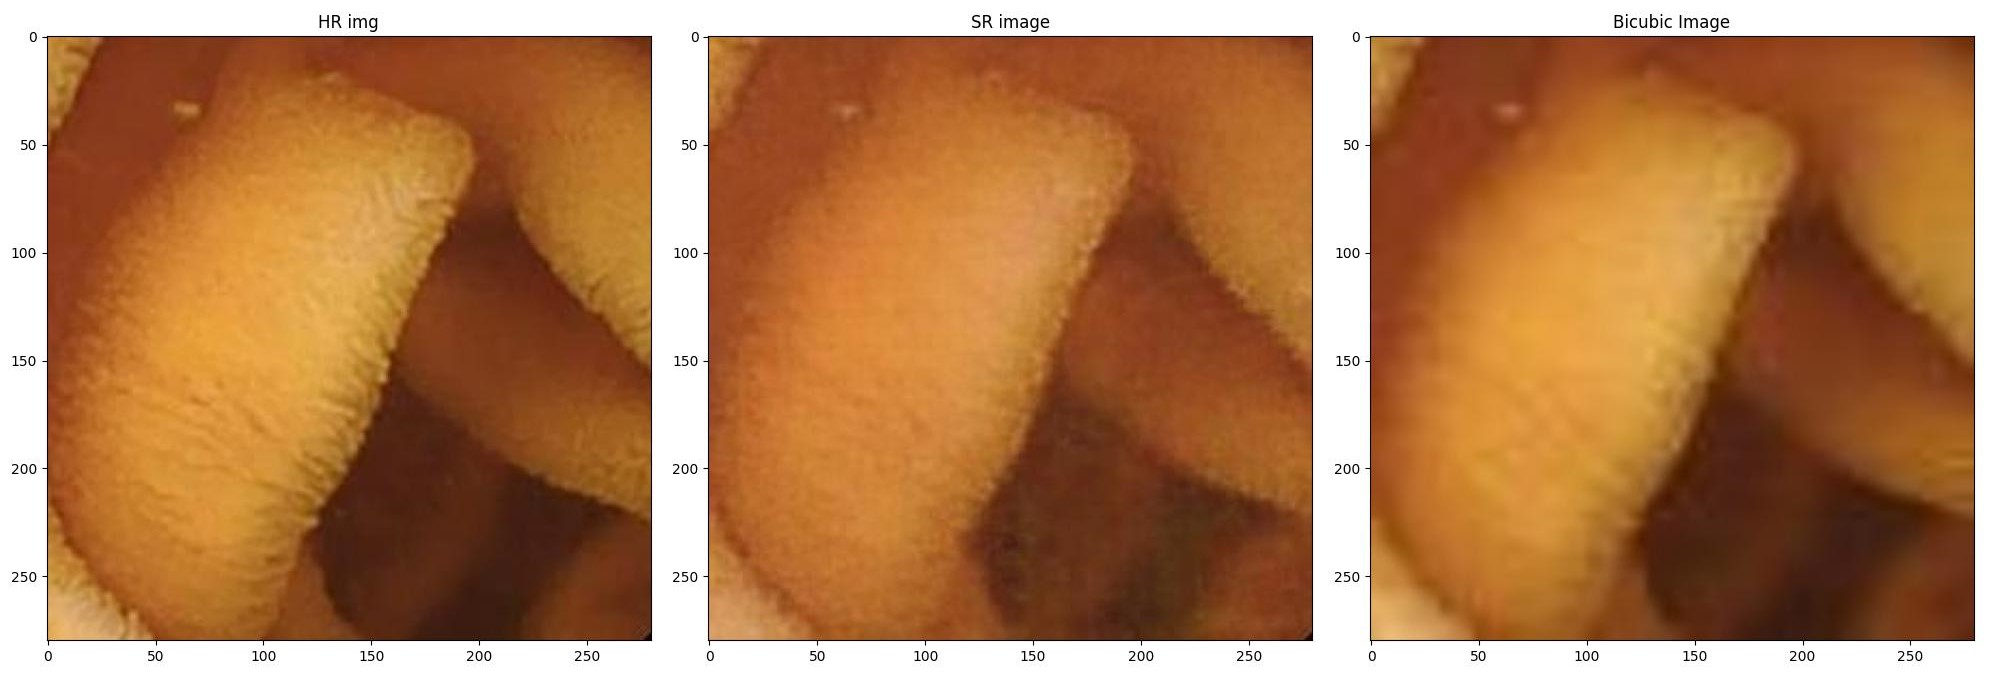
\includegraphics[totalheight=1.8in]{Chapter5/cropped_test (12).jpg}
%    \vspace{0.1}
%    \includegraphics[totalheight=1.8in]{Chapter5/cropped_test %(12)_SSIM.jpg}
%    \caption[CycleGAN Generated Image and their SSIM maps]{SRGAN Generated %Image and their SSIM maps: (1) HR image (2) SR image (3)Bicubic %Interpolated image (4) SSIM-map (HR-SR) (5) SSIM-map (HR-Bicubic) (6) %SSIM-map (SR-Bicubic)\cite{CycleGAN} \cite{SSIM}}
%    \label{fig:label5.7}
%\end{figure}

\subsection{Training details of SR-Densenet}
Non-overlapping sub-images with a size of 336 × 336 were cropped in the HR space. The LR images were obtained by downsampling the HR images using bicubic kernel with a scale factor of 4×. Each image has been transformed into YCbCr space and only the Y-channel was used for training. In all networks, 8 DenseNet blocks were used, resulting in 64 convolution layers. Within each block, a growth rate of 16 was set. This generated an output of 128 feature maps from each block. The filter size was set to 3 × 3 in all weight layers. The rectified linear units (ReLu) was used as the activation function. All the networks were optimized using Adam. The learning rate was initially set to 0.0001. A mini-batch size of 32 was set during the training. The training process stopped after no improvements of the loss was observed after 200 epoches.
\begin{table}[H]
\centering
\caption{PSNR and SSIM for SR Densenet.}
\begin{tabular}{ |c|c|c|c| }
\hline
 Method & PSNR(dB) & SSIM(dB) & Dataset \\ 
  \hline
 BICUBIC &	35.36 &	0.88 & uncropped \\
 SR Densenet &	32 &	0.925 & uncropped \\
 BICUBIC &	37.2 &	0.9 & cropped \\
 SR Densenet &	38.86	& 0.92 & cropped\\
\hline
\end{tabular}
\label{Table:5.3}
\end{table}
\begin{figure}[H]
    \centering
    \begin{subfigure}[b]{0.275\textwidth}
    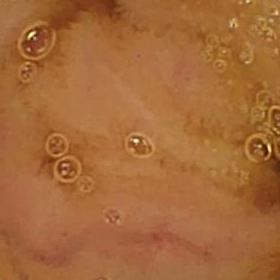
\includegraphics[width=\textwidth]{Chapter7/hr_9.jpg}
    \caption{HR}
  \end{subfigure}
  \begin{subfigure}[b]{0.275\textwidth}
    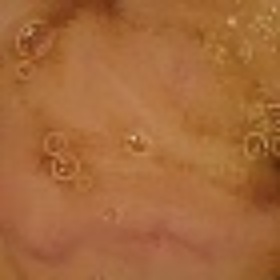
\includegraphics[width=\textwidth]{Chapter7/Bicubic_9.jpg}
    \caption{Bicubic}
  \end{subfigure}
  \begin{subfigure}[b]{0.275\textwidth}
    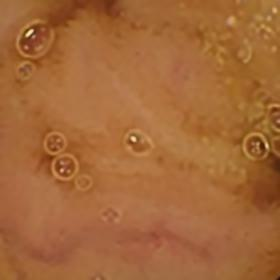
\includegraphics[width=\textwidth]{Chapter7/Dense_9.jpg}
    \caption{DenseNET}
  \end{subfigure}
  
  \begin{subfigure}[b]{0.275\textwidth}
    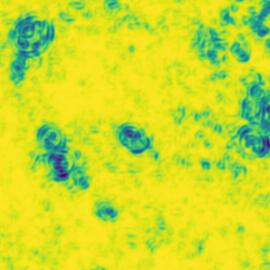
\includegraphics[width=\textwidth]{Chapter7/SSIM_bicubic_9.jpg}
    \caption{HR-Bicubic}
  \end{subfigure}
  \begin{subfigure}[b]{0.275\textwidth}
    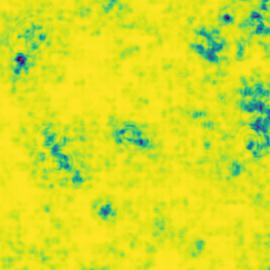
\includegraphics[width=\textwidth]{Chapter7/SSIM_densenet_9.jpg}
    \caption{HR-DenseNET}
  \end{subfigure}
    \caption{SR Densenet Generated Image}{SR Densenet Generated Image and their SSIM maps.\cite{DenseNET} \cite{SSIM}}
    \label{fig:test23}
\end{figure}

\subsection{Training details of RCAN}
10,000 training images Kvasir Capsule Endoscopy were used as training set. Experiments with conducted using bicubic images. The SR results were evaluated with PSNR and SSIM on Y channel of transformed YCbCr space. Data augmentation is performed on the 10,000 training images, which are randomly rotated by 90 , 180 , 270 degrees and flipped horizontally. In each training batch, 16 LR color patches with the size of 48 × 48 are extracted as inputs. Model is trained by adam optimizer. The initial leaning rate was set to 0.0001 and then decreases to half every 2 × 100000 iterations of back-propagation. PyTorch was used to implement our models.  

\begin{table}[H]
\subsection{Results of RCAN}
\centering
\caption{PSNR and SSIM for RCAN.}
\begin{tabular}{ |c|c|c|c| }
\hline
 Method & PSNR(dB) & SSIM(dB) & Dataset \\ 
  \hline
 BICUBIC &	35.36 &	0.88 & uncropped \\
 RCAN &	31.8 &	0.91 & uncropped \\
 BICUBIC &	37.1 &	0.89 & cropped \\
 RCAN &	39.47	& 0.92 & cropped\\
\hline
\end{tabular}
\label{Table:5.3}
\end{table}
\begin{figure}[H]
    \centering
        \begin{subfigure}[b]{0.275\textwidth}
    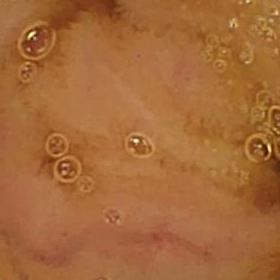
\includegraphics[width=\textwidth]{Chapter7/hr_9.jpg}
    \caption{HR}
  \end{subfigure}
  \begin{subfigure}[b]{0.275\textwidth}
    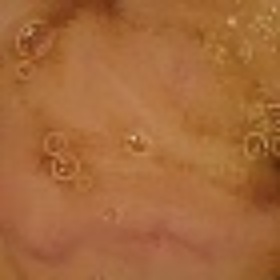
\includegraphics[width=\textwidth]{Chapter7/Bicubic_9.jpg}
    \caption{Bicubic}
  \end{subfigure}
  \begin{subfigure}[b]{0.275\textwidth}
    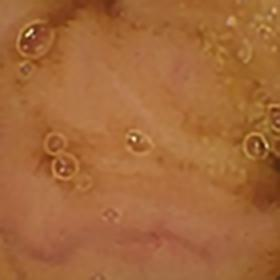
\includegraphics[width=\textwidth]{Chapter7/rcan_9.jpg}
    \caption{RCAN}
  \end{subfigure}
  
  \begin{subfigure}[b]{0.275\textwidth}
    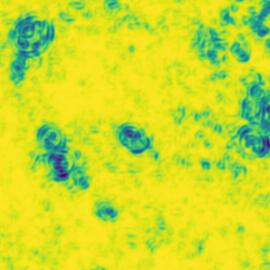
\includegraphics[width=\textwidth]{Chapter7/SSIM_bicubic_9.jpg}
    \caption{HR-Bicubic}
  \end{subfigure}
  \begin{subfigure}[b]{0.275\textwidth}
    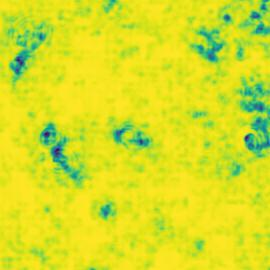
\includegraphics[width=\textwidth]{Chapter7/SSIM_rcan_9.jpg}
    \caption{HR-RCAN}
  \end{subfigure}
    \caption{RCAN generated images}{RCAN Generated Image and their SSIM maps: (1) HR image (2) Bicubic Interpolated image (3) SR image (4)  SSIM-map (HR-Bicubic) (5)SSIM-map (HR-SR) }
    \label{fig:test23}
\end{figure}

\section{Experimental Analysis on proposed models}
The results obtained from each model is shown subsequent figures.
Fig \ref{fig:label7.1} shows the images from cycleCNN on mse loss and Fig \ref{fig:label7.2} shows the images from dense cycleCNN training. Fig \ref{fig:label7.3} shows images from dense cycleCNN on Y channel of YCbCr scolour space and Fig \ref{fig:label7.4} represents the images generated by training the dense cycleCNN network on patch of 100x100 pixels.

\begin{figure}[H]
    \centering

    \begin{subfigure}[b]{0.32\textwidth}
    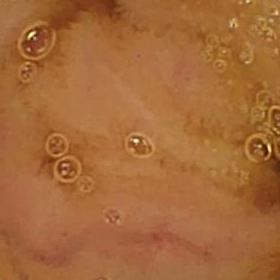
\includegraphics[width=\textwidth]{Chapter7/hr_9.jpg}
    \caption{Original}
  \end{subfigure}
  \begin{subfigure}[b]{0.32\textwidth}
    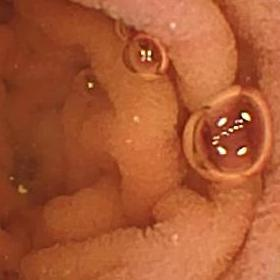
\includegraphics[width=\textwidth]{Chapter7/hr_445.jpg}
    \caption{Original}
  \end{subfigure}
  \begin{subfigure}[b]{0.32\textwidth}
    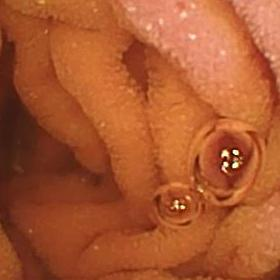
\includegraphics[width=\textwidth]{Chapter7/hr_456.jpg}
    \caption{Original}
  \end{subfigure}

    \begin{subfigure}[b]{0.32\textwidth}
    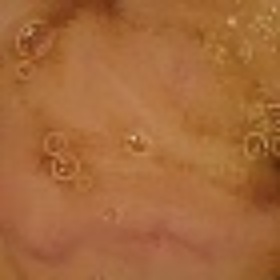
\includegraphics[width=\textwidth]{Chapter7/Bicubic_9.jpg}
    \caption{Bicubic}
  \end{subfigure}
  \begin{subfigure}[b]{0.32\textwidth}
    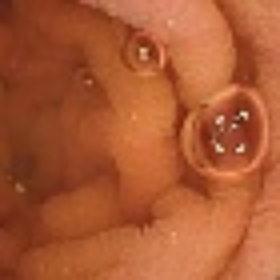
\includegraphics[width=\textwidth]{Chapter7/Bicubic_445.jpg}
    \caption{Bicubic}
  \end{subfigure}
  \begin{subfigure}[b]{0.32\textwidth}
    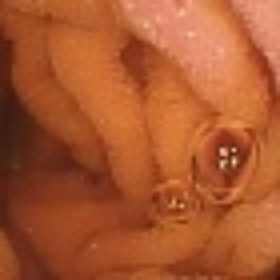
\includegraphics[width=\textwidth]{Chapter7/Bicubic_456.jpg}
    \caption{Bicubic}
  \end{subfigure}
  
  \begin{subfigure}[b]{0.32\textwidth}
    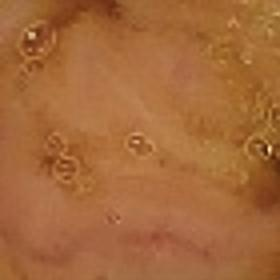
\includegraphics[width=\textwidth]{Chapter7/cycle_mse_9.jpg}
    \caption{Cycle MSE}
  \end{subfigure}
  \begin{subfigure}[b]{0.32\textwidth}
    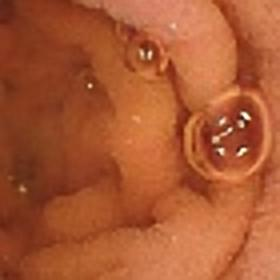
\includegraphics[width=\textwidth]{Chapter7/cycle_mse_445.jpg}
    \caption{Cycle MSE}
  \end{subfigure}
  \begin{subfigure}[b]{0.32\textwidth}
    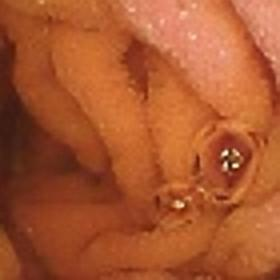
\includegraphics[width=\textwidth]{Chapter7/cycle_mse_456.jpg}
    \caption{Cycle MSE}
  \end{subfigure}
    
    \caption[Images generated using MSE loss on CycleCNN Model.]{Images generated using MSE loss on CycleCNN Model.}
    \label{fig:label7.1}
\end{figure}


\begin{figure}[H]
    \centering
        \begin{subfigure}[b]{0.32\textwidth}
    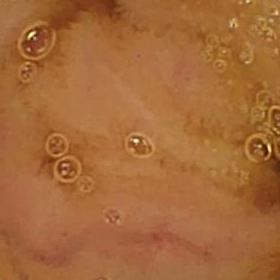
\includegraphics[width=\textwidth]{Chapter7/hr_9.jpg}
    \caption{Original}
  \end{subfigure}
  \begin{subfigure}[b]{0.32\textwidth}
    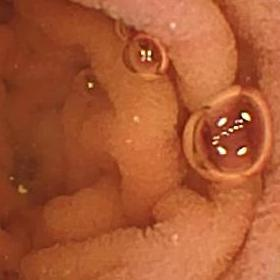
\includegraphics[width=\textwidth]{Chapter7/hr_445.jpg}
    \caption{Original}
  \end{subfigure}
  \begin{subfigure}[b]{0.32\textwidth}
    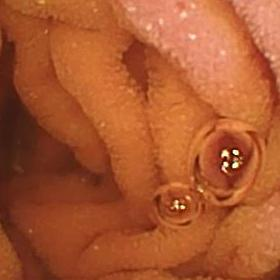
\includegraphics[width=\textwidth]{Chapter7/hr_456.jpg}
    \caption{Original}
  \end{subfigure}

    \begin{subfigure}[b]{0.32\textwidth}
    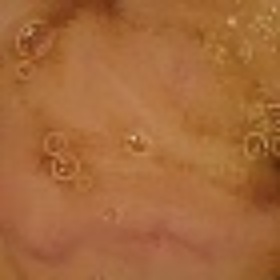
\includegraphics[width=\textwidth]{Chapter7/Bicubic_9.jpg}
    \caption{Bicubic}
  \end{subfigure}
  \begin{subfigure}[b]{0.32\textwidth}
    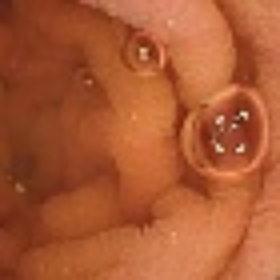
\includegraphics[width=\textwidth]{Chapter7/Bicubic_445.jpg}
    \caption{Bicubic}
  \end{subfigure}
  \begin{subfigure}[b]{0.32\textwidth}
    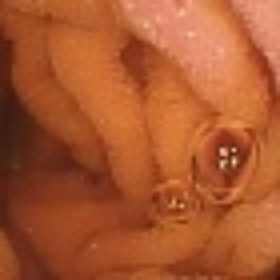
\includegraphics[width=\textwidth]{Chapter7/Bicubic_456.jpg}
    \caption{Bicubic}
  \end{subfigure}
  
  \begin{subfigure}[b]{0.32\textwidth}
    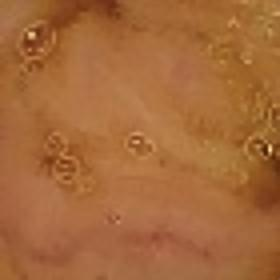
\includegraphics[width=\textwidth]{Chapter7/dense_grl_9.jpg}
    \caption{Dense GRL}
  \end{subfigure}
  \begin{subfigure}[b]{0.32\textwidth}
    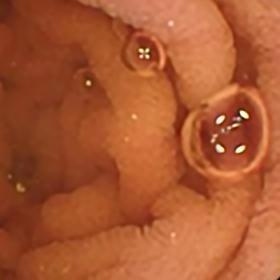
\includegraphics[width=\textwidth]{Chapter7/Dense_445.jpg}
    \caption{Dense GRL}
  \end{subfigure}
  \begin{subfigure}[b]{0.32\textwidth}
    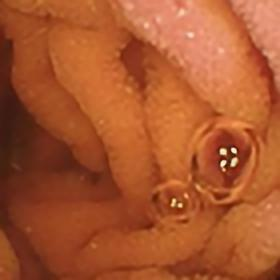
\includegraphics[width=\textwidth]{Chapter7/Dense_456.jpg}
    \caption{Dense GRL}
  \end{subfigure}
    \caption[Images generated Dense CycleCNN Model with GRL Block.]{Images generated Dense CycleCNN Model with GRL Block.}
    \label{fig:label7.2}
\end{figure}
It can be observed that the images generated using dense connections and GRL block are visually more better than the traditional bicubic interpolation method. In bicubic interpolation blur effect is introduced and the high frequency details are not captured, while using this architecture we are able to capture high frequency details efficiently.

\begin{figure}[H]
    \centering

    \begin{subfigure}[b]{0.32\textwidth}
    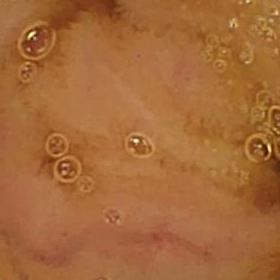
\includegraphics[width=\textwidth]{Chapter7/hr_9.jpg}
    \caption{Original}
  \end{subfigure}
  \begin{subfigure}[b]{0.32\textwidth}
    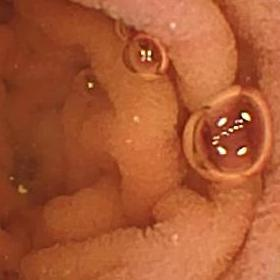
\includegraphics[width=\textwidth]{Chapter7/hr_445.jpg}
    \caption{Original}
  \end{subfigure}
  \begin{subfigure}[b]{0.32\textwidth}
    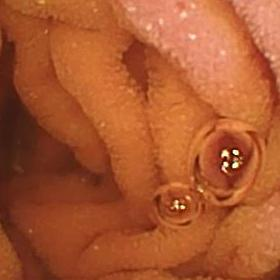
\includegraphics[width=\textwidth]{Chapter7/hr_456.jpg}
    \caption{Original}
  \end{subfigure}

    \begin{subfigure}[b]{0.32\textwidth}
    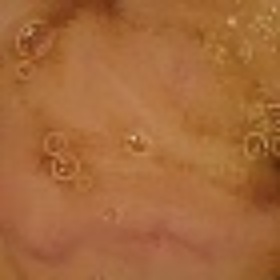
\includegraphics[width=\textwidth]{Chapter7/Bicubic_9.jpg}
    \caption{Bicubic}
  \end{subfigure}
  \begin{subfigure}[b]{0.32\textwidth}
    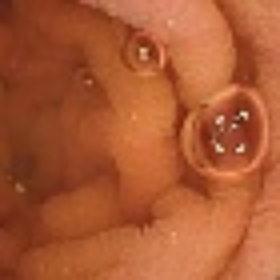
\includegraphics[width=\textwidth]{Chapter7/Bicubic_445.jpg}
    \caption{Bicubic}
  \end{subfigure}
  \begin{subfigure}[b]{0.32\textwidth}
    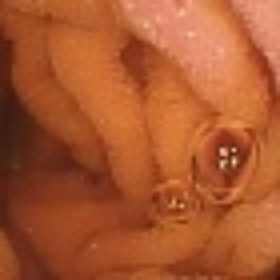
\includegraphics[width=\textwidth]{Chapter7/Bicubic_456.jpg}
    \caption{Bicubic}
  \end{subfigure}
  
  \begin{subfigure}[b]{0.32\textwidth}
    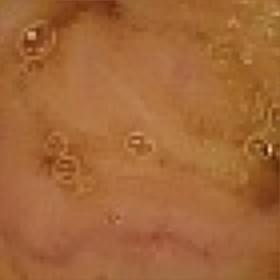
\includegraphics[width=\textwidth]{Chapter7/Ycbcr_cycle_dense_9.jpg}
    \caption{DenseGRL YCbCr}
  \end{subfigure}
  \begin{subfigure}[b]{0.32\textwidth}
    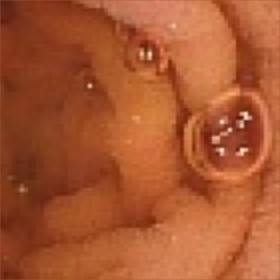
\includegraphics[width=\textwidth]{Chapter7/Ycbcr_cycle_dense_445.jpg}
    \caption{DenseGRL YCbCr}
  \end{subfigure}
  \begin{subfigure}[b]{0.32\textwidth}
    \includegraphics[width=\textwidth]{Chapter7/Ycbcr_cycle_dense_456.jpg}
    \caption{DenseGRL YCbCr}
  \end{subfigure}
    
    \caption[Images generated Dense CycleCNN Model with GRL Block on YCbCr.]{Images generated Dense CycleCNN Model with GRL Block on YCbCr.}
    \label{fig:label7.3}
\end{figure}

While training on Y-channel of YCbCr colour space, the network is able to out-perform the traditional bicubic approach and the results are quite similar to that of training done on RGB colour space. The advantage we gain here is the reduced training parameters and faster training of model.


\begin{figure}[H]
    \centering

        \begin{subfigure}[b]{0.32\textwidth}
    \includegraphics[width=\textwidth]{Chapter7/hr_9.jpg}
    \caption{Original}
  \end{subfigure}
  \begin{subfigure}[b]{0.32\textwidth}
    \includegraphics[width=\textwidth]{Chapter7/hr_445.jpg}
    \caption{Original}
  \end{subfigure}
  \begin{subfigure}[b]{0.32\textwidth}
    \includegraphics[width=\textwidth]{Chapter7/hr_456.jpg}
    \caption{Original}
  \end{subfigure}

    \begin{subfigure}[b]{0.32\textwidth}
    \includegraphics[width=\textwidth]{Chapter7/Bicubic_9.jpg}
    \caption{Bicubic}
  \end{subfigure}
  \begin{subfigure}[b]{0.32\textwidth}
    \includegraphics[width=\textwidth]{Chapter7/Bicubic_445.jpg}
    \caption{Bicubic}
  \end{subfigure}
  \begin{subfigure}[b]{0.32\textwidth}
    \includegraphics[width=\textwidth]{Chapter7/Bicubic_456.jpg}
    \caption{Bicubic}
  \end{subfigure}
  
  \begin{subfigure}[b]{0.32\textwidth}
    \includegraphics[width=\textwidth]{Chapter7/patch_ycbcr_dense_9.jpg}
    \caption{Patch Dense CycleCNN(YCbCr)}
  \end{subfigure}
  \begin{subfigure}[b]{0.32\textwidth}
    \includegraphics[width=\textwidth]{Chapter7/patch_ycbcr_dense_445.jpg}
    \caption{Patch Dense CycleCNN(YCbCr)}
  \end{subfigure}
  \begin{subfigure}[b]{0.32\textwidth}
    \includegraphics[width=\textwidth]{Chapter7/patch_ycbcr_dense_456.jpg}
    \caption{Patch Dense CycleCNN(YCbCr)}
  \end{subfigure}
    
    \caption[Images generated Dense CycleCNN Model with GRL Block on YCbCr with patch.]{Images generated Dense CycleCNN Model with GRL Block on YCbCr with patch.}
    \label{fig:label7.4}
\end{figure}
On training the network on patch size of 100x100 and Y-channel of YCbCr colour space, the network is able to beat the traditional bicubic approach and the results are similar to that of training done on RGB colour space and while image of 280x280 pixels. The advantage we gain here is faster training of model and low memory consumption.
\subsection{DenseNET with Channel Attention Block(DCAN)}


\begin{figure}[H]
  \centering
  \begin{subfigure}[b]{0.275\textwidth}
    \includegraphics[width=\textwidth]{Chapter7/Bicubic_9.jpg}
    \caption{Bicubic}
  \end{subfigure}
  \begin{subfigure}[b]{0.275\textwidth}
    \includegraphics[width=\textwidth]{Chapter7/Bicubic_445.jpg}
    \caption{Bicubic}
  \end{subfigure}
  \begin{subfigure}[b]{0.275\textwidth}
    \includegraphics[width=\textwidth]{Chapter7/Bicubic_456.jpg}
    \caption{Bicubic}
  \end{subfigure}
  
  \begin{subfigure}[b]{0.275\textwidth}
    \includegraphics[width=\textwidth]{Chapter7/srgan_9.jpg}
    \caption{SRGAN}
  \end{subfigure}
  \begin{subfigure}[b]{0.275\textwidth}
    \includegraphics[width=\textwidth]{Chapter7/srgan_445.jpg}
    \caption{SRGAN}
  \end{subfigure}
  \begin{subfigure}[b]{0.275\textwidth}
    \includegraphics[width=\textwidth]{Chapter7/srgan_456.jpg}
    \caption{SRGAN}
  \end{subfigure}
  
  \begin{subfigure}[b]{0.275\textwidth}
    \includegraphics[width=\textwidth]{Chapter7/Dense_9.jpg}
    \caption{DenseNET}
  \end{subfigure}
  \begin{subfigure}[b]{0.275\textwidth}
    \includegraphics[width=\textwidth]{Chapter7/Dense_445.jpg}
    \caption{DenseNET}
  \end{subfigure}
  \begin{subfigure}[b]{0.275\textwidth}
    \includegraphics[width=\textwidth]{Chapter7/Dense_456.jpg}
    \caption{DenseNET}
  \end{subfigure}

    \begin{subfigure}[b]{0.275\textwidth}
    \includegraphics[width=\textwidth]{Chapter7/rcan_9.jpg}
    \caption{RCAN}
  \end{subfigure}
  \begin{subfigure}[b]{0.275\textwidth}
    \includegraphics[width=\textwidth]{Chapter5/rcan_445.jpg}
    \caption{RCAN}
  \end{subfigure}
  \begin{subfigure}[b]{0.275\textwidth}
    \includegraphics[width=\textwidth]{Chapter7/rcan_456.jpg}
    \caption{RCAN}
  \end{subfigure}
  
     \begin{subfigure}[b]{0.275\textwidth}
    \includegraphics[width=\textwidth]{Chapter7/DCAN_9.jpg}
    \caption{DCAN Image(ours)}
  \end{subfigure}
  \begin{subfigure}[b]{0.275\textwidth}
    \includegraphics[width=\textwidth]{Chapter7/Dense_445.jpg}
    \caption{DCAN Image(ours)}
  \end{subfigure}
  \begin{subfigure}[b]{0.275\textwidth}
    \includegraphics[width=\textwidth]{Chapter7/DCAN_456.jpg}
    \caption{DCAN Image(ours)}
  \end{subfigure}
  
  \caption{Comparison of images of proposed network with State of Art models}
  \label{fig:DCAN}
\end{figure}

The training is done to minimize the loss function which is the taken as the Mean Squared Loss(MSE). The training is completed for a total of 300 epochs with a batch size of 32. We did the training on patch of image, each of size 100x100, and on the Y channel of YCbCr channel. We already illustrated the benifits of training on patch of image and Y channel of YCbCr above. Adam optimizer with a learning rate of 0.0001. The quantitative analysis and qualitative analysis of the proposed model (DCAN) is shown in upcoming sections.


The results obtained after training of proposed model as well as its comparison with state of art models is shown in Fig. \ref{fig:DCAN} After obtaining results from different proposed models, images from each model were evaluated on different image quality matrices to carry out the comparison.
The SSIM maps for each image is shown in Fig. \ref{fig:label7.6}, Fig. \ref{fig:label7.7}

\begin{figure}[H]
    \centering
    \begin{subfigure}[H]{0.275\textwidth}
    \includegraphics[width=\textwidth]{Chapter7/hr_445.jpg}
    \caption{Original HR Image}
  \end{subfigure}
  \begin{subfigure}[H]{0.275\textwidth}
    \includegraphics[width=\textwidth]{Chapter7/SSIM_bicubic_445.jpg}
    \caption{HR Bicubic}
  \end{subfigure}
  \begin{subfigure}[H]{0.275\textwidth}
    \includegraphics[width=\textwidth]{Chapter7/SSIM_srgan_445.jpg}
    \caption{HR-SRGAN}
  \end{subfigure}
  
  \begin{subfigure}[H]{0.275\textwidth}
    \includegraphics[width=\textwidth]{Chapter7/SSIM_densenet_445.jpg}
    \caption{HR-SRDensenet}
  \end{subfigure}
  \begin{subfigure}[H]{0.275\textwidth}
    \includegraphics[width=\textwidth]{Chapter7/SSIM_rcan_445.jpg}
    \caption{HR-RCAN}
  \end{subfigure}
  \begin{subfigure}[H]{0.275\textwidth}
    \includegraphics[width=\textwidth]{Chapter7/SSIM_proposed_445.jpg}
    \caption{HR-Proposed}
  \end{subfigure}

    
    \caption[SSIM maps for images generated form different models.] {SSIM maps for Images generated from different models. Yellow region shows similarity while the blue region shows dissimilarity.}
    \label{fig:label7.6}
\end{figure}




It can be observed from the SSIM maps that the our model is able to beat the state of art models like SRDensenet and RCAN. Our model exceptionally well and their outputs are very close to ground truth images.

\begin{figure}[H]
    \centering

    \begin{subfigure}[b]{0.275\textwidth}
    \includegraphics[width=\textwidth]{Chapter7/hr_9.jpg}
    \caption{Original HR Image}
  \end{subfigure}
  \begin{subfigure}[b]{0.275\textwidth}
    \includegraphics[width=\textwidth]{Chapter7/SSIM_bicubic_9.jpg}
    \caption{HR Bicubic}
  \end{subfigure}
  \begin{subfigure}[b]{0.275\textwidth}
    \includegraphics[width=\textwidth]{Chapter7/SSIM_srgan_9.jpg}
    \caption{HR-SRGAN}
  \end{subfigure}
  
  \begin{subfigure}[b]{0.275\textwidth}
    \includegraphics[width=\textwidth]{Chapter7/SSIM_densenet_9.jpg}
    \caption{HR-SRDensenet}
  \end{subfigure}
  \begin{subfigure}[b]{0.275\textwidth}
    \includegraphics[width=\textwidth]{Chapter7/SSIM_rcan_9.jpg}
    \caption{HR-RCAN}
  \end{subfigure}
  \begin{subfigure}[b]{0.275\textwidth}
    \includegraphics[width=\textwidth]{Chapter7/SSIM_proposed_9_marked.png}
    \caption{HR-Proposed}
  \end{subfigure}
    
    \caption[SSIM maps for images generated form different models.] {SSIM maps for Images generated from different models:
    (1) Original HR image (2) HR-Bicubic (3) HR-SRGAN (4) HR-SRDensenet (5) HR-RCAN (6) HR-Propsed (Yellow region shows similarity while the blue region shows disimilarity.)}
    \label{fig:label7.7}
\end{figure}


\begin{figure}[H]{\textwidth}
    \centering
    \includegraphics[width=\textwidth]{Chapter7/Patch Analysis.png}
    \caption[Patch Analysis]{Patch Analysis}
    \label{fig:label7.8}
\end{figure}



Analysis on the patch showed in Fig. \ref{fig:label7.7} can be shown in Fig. \ref{fig:label7.8} The right side of the image shows the patch extracted from different models such as proposed model, srgan model, rcan model, densenet model, and bicubic interpolation. The left side displays the SSIM map for the corresponding region of each image.






\section{Quantitative Analysis}
The average SSIM and PSNR values for the testing images of each model is provided in table \ref{Table:6.1}

\begin{table}[H]
    \centering
    \caption{PSNR, SSIM and LPIPS of all models.}
\begin{tabular}{|c c c c|}
  \hline
   \begin{tabular}{|c|}
        Model \\
        \hline
          \\
        Proposed \\
        \hline
        Bicubic \\
        \hline
        SRGAN \cite{SRGAN}\\
        \hline
        DenseNET \cite{DenseNET} \\
        \hline
        RCAN\cite{RCAN}\\
        \hline
        CycleCNN(MSE) \\
        \hline
        Dense CycleCNN(GRL) \\
        \hline
        YCbCr CycleCNN \\
        \hline
        Patch CycleCNN \\
        \hline
        \end{tabular}    
        & \begin{tabular}{|c|c|}
        \multicolumn{2}{|c|}{PSNR $\uparrow$}\\
        \hline
        Y-Channel & RGB \\
        \hline
        40.2261 $\uparrow$ & 39.5389 $\uparrow$ \\
        \hline
        38.1069 & 37.2111 \\
        \hline
        38.0377 & 37.0021 \\
        \hline
        39.6842 & 38.8596 \\
        \hline
        40.1438 & 39.4613\\
        \hline
        38.0121 & 37.0143 \\
        \hline
        38.1546 & 37.1453 \\
        \hline
        36.4098 & 35.5234 \\
        \hline
        36.6342 & 35.7452 \\
        \hline
        \end{tabular}  & \begin{tabular}{|c|c|}
        \multicolumn{2}{|c|}{SSIM $\uparrow$}\\
        \hline
        Y-Channel & RGB \\
        \hline
        0.9486 $\uparrow$ & 0.9378 $\uparrow$ \\
        \hline
        0.9296 & 0.9057 \\
        \hline
        0.9291 & 0.9049 \\
        \hline
        0.9401 & 0.9369 \\
        \hline
        0.9427 & 0.9371\\
        \hline
        0.9102 & 0.9012 \\
        \hline
        0.9013 & 0.8912 \\
        \hline
        0.8991 & 0.8993 \\
        \hline
        0.9015 & 0.9023 \\
        \hline
        \end{tabular}  & \begin{tabular}{|c|}
        LPIPS $\downarrow$\\
        \hline
        RGB \\
        \hline
        0.1346 $\downarrow$\\
        \hline
         0.2310\\
        \hline
         0.1972\\
        \hline
        0.1353 \\
        \hline
        0.1359 \\
        \hline
        0.1982 \\
        \hline
        0.1895 \\
        \hline
        0.1783 \\
        \hline
        0.1732 \\
        \hline
        \end{tabular} \\
    \hline
\end{tabular}
\label{Table:6.1}
\end{table}

It can be observed that the PSNR and SSIM values of the proposed model are high compared to the present State of Art models, such as SR-Densenet and RCAN. The LPIPS values are also the lowest. Proposed model is providing the best values for all the image quality assessment metrices taken under consideration namely PSNR, SSIM and LPIPS. 
\subsection{Statistical Analysis}

Statistical analysis was also conducted on the results of the proposed model to ensure the model consistency compared to SOTA models. The values of standard deviation of each model are presented in table \ref{Table:7.1}       

\begin{table}[H]
\centering
\caption{Standard Deviation Values}
\begin{tabular}{ |c|c| }
\hline
 Model & Standard deviation \\ 
  \hline
 Proposed &	2.0186\\
 \hline
 BICUBIC & 2.2102\\
 \hline
 SRGAN \cite{SRGAN} &  2.6924\\
 \hline
 DenseNET \cite{DenseNET} & 3.1996\\
 \hline
 RCAN \cite{RCAN} &	 2.8753\\
 \hline
\end{tabular}
\label{Table:7.1}
\end{table}

Box plots were used to observe the spread and outliers of the PSNR and SSIM values of proposed model. They are present in the Fig. \ref{fig:label7.9}

\begin{figure}[H]
    \centering

    \begin{subfigure}[b]{0.275\textwidth}
    \includegraphics[width=\textwidth]{Chapter7/proposed_y.png}
    \caption{Proposed}
  \end{subfigure}
  \begin{subfigure}[b]{0.275\textwidth}
    \includegraphics[width=\textwidth]{Chapter7/bicubic_y.png}
    \caption{Bicubic}
  \end{subfigure}
  \begin{subfigure}[b]{0.275\textwidth}
    \includegraphics[width=\textwidth]{Chapter7/srgan_y.png}
    \caption{SRGAN}
  \end{subfigure}
  
  \begin{subfigure}[b]{0.275\textwidth}
    \includegraphics[width=\textwidth]{Chapter7/rcan_y.png}
    \caption{RCAN}
  \end{subfigure}
  \begin{subfigure}[b]{0.275\textwidth}
    \includegraphics[width=\textwidth]{Chapter7/dense_y.png}
    \caption{DenseNET}
  \end{subfigure}
 
    
    \caption[Box plots for different models.] {Box plots for different models}
    \label{fig:label7.9}
\end{figure}
We can clearly observe that the proposed model is more consistent owing to the lower standard deviation and the lower number of outlier compared to the other SOTA models.  



